So versuchen wir uns also am Führen eines Lerntagebuchs. In Zeiten von COVID-19 ist es uns nicht gegeben persönlich zu Veranstaltungen zu erscheinen.
Das bietet Vor- aber auch Nachteile. So hängt der persönliche Lernerfolg noch mehr als vorher an einem selbst, der eigenen Motivation, dem Interesse
Thema und dem omnipräsenten Schweinehund. Vorteilhaft unter anderem sehe ich das Führen dieses Tagebuchs. Interesse für die Dinge jenseits des
Tellerrandes waren schon immer legitim, gar geboten. Durch den Wegfall der Klausur und dem damit verbundenen zielstrebigen lernen auf \textit{Klausurrelevantes}
erscheint es plötzlich aber auch tatsächlich machbar.\\
Wie gesagt - erscheint. Wir befinden uns derzeit in der dritten Semesterwoche und die meisten Veranstaltungen beginnen gerade erst anzuziehen - 
für endgültige Urteile schätze ich ist es also noch etwas zu früh.\\\\
Es handelt sich hier um die erste Veranstaltung WT1 und wir sind noch nicht super tief in die Materie (pun intended) eingestiegen. Vieles, was bisher
vermittelt wurde ist also noch recht basic. Es war allerdings auch neues dabei. So erscheint es mir immernoch etwas kontraintuitiv, dass kristalline Festkörper
eine höhere (laut Skript \textbf{die} höchste) Atomdichte als amorphe haben sollen. Streben kristalline Strukturen nach der dichtesten Packung?
Wenn dem so ist, warum tuhen es ihnen amorphe Strukturen nicht gleich? Zumindest was die Tatsache, dass ein kristallines Atomgitter dichter ist, als ein amorphe
Anordnung ist konnte eine kurze Internetrecherche verdeutlichen. Die zweite Frage bleibt allerdings noch bestehen. In Bezug auf Moleküle kann ich es mir noch recht
erklären. Molekulare Dipole haben eine räumliche Geometrie und eine Vorzugsrichtung, in der sie sich anordnen. Elementar vorliegende Materialien aber?
Es muss irgend eine Kraft geben die verhindert, dass die Atome enger aneinander Rücken. Und wenn diese Kraft überwunden wurde, warum verbleiben einige Elemente dann
in der Konfiguration gegen die sie sich so sehr gewehrt haben (Kohlenstoff - Graphit, Diamant, Trockeneis, Gas ...)?\\
Wenn das beteiligte Element innerhalb eines Materials gleich gehalten wird wärend seine kristalline Konfiguration variiert wird ändern sich seine physikalischen Eigenschaften.
So zumindest das Statement des Skriptes. Das deckt sich auch mit eigenen Beobachtungen in der realen Welt. Wer schon mal versucht hat ein Blech aus gewalztem Stahl zu
scheren wird bemerken, dass es in Walzrichtung deutlich einfacher funktioniert. Das hat einen ähnlichen Effekt wie beim Versuch ein Taschentuch entlang einer Kante 
oder der orthogonal zu ihr liegenden zu reißen.\\
Sobald die Bücher aus der Bib da sind werde ich Recherche betreiben müssen was die im Skript erwähnten Bravais-Gitter angeht. Bezogen auf Metalle
soll es maximal sieben verschiedene Achsenkreuze geben aus denen wiederum 14 verschiedene Bravais-Gitter ableitbar sind. Eine recht gute bildliche Darstellung
aller 14 Bravais-Gitter ließ sich recht schnell im Netz finden.

\begin{figure}[H]
    \centering
    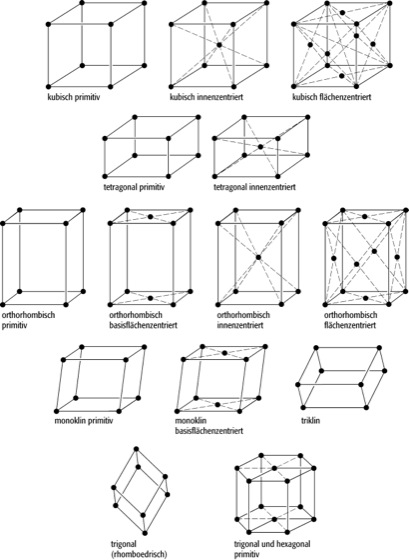
\includegraphics[width=0.7\textwidth]{entries/1/bravais.jpg}
    \caption{Bravais-Gitter, Quelle: https://www.spektrum.de/lexikon/physik/bravais-gitter/1948}
\end{figure}

Über die Konstruktion der Achsenkreuze und der daraus resultierenden Gitterstrukturen muss ich mir allerdings noch etwas mehr Gedanken machen. 
Es wundert mich überhaupt nicht, dass es zum Thema Topologie in der Mathematik eine ganze Unterdisziplin gibt.\\
Möglicherweise findet sich ein Tool, welches den Aufbau 3-dimensional darstellt?